\documentclass{article}
\usepackage[paperwidth=210mm,paperheight=297mm, top = 30mm, bottom = 30mm]{geometry}
%\usepackage[hangul]{kotex}
\usepackage{kotex}
\usepackage[utf8]{inputenc}
\usepackage{enumitem}
\usepackage{indentfirst}
\usepackage{graphicx, subcaption, tikz, pgfplots}
\usepackage{amsmath, amssymb, amsthm, amsfonts, bm}
\usepackage{listings}
\usepackage{mathrsfs}
\usetikzlibrary{arrows}
\pgfplotsset{compat=1.15}

\title{2020 Spring MAS365 Numerical Analysis HW6}
\author{20160650 채지석}
\date{\today}

\setlist{  
  listparindent=\parindent,
  %parsep=0pt,
}

\lstset{frame=tb,
  language=Python,
  aboveskip=3mm plus 2mm,
  belowskip=3mm plus 2mm minus 2mm,
  showstringspaces=false,
  columns=flexible,
  basicstyle={\small\ttfamily},
  numbers=none,
  %numberstyle=\tiny\color{gray},
  %keywordstyle=\color{blue},
  %commentstyle=\color{dkgreen},
  %stringstyle=\color{mauve},
  breaklines=true,
  breakatwhitespace=true,
  frame=single,
  tabsize=4
}

\newtheorem{prob}{Problem}

\newcommand{\set}[1]{\left\{ {#1} \right\}}
\newcommand{\vecx}{\boldsymbol{x}}
\newcommand{\mat}[1]{\boldsymbol{#1}}
\newcommand{\mata}{\boldsymbol{A}}
\newcommand{\matb}{\boldsymbol{B}}
\newcommand{\rr}{\mathbb{R}}
\newcommand{\nn}{\mathbb{N}}
\newcommand{\zz}{\mathbb{Z}}
\newcommand{\cc}{\mathbb{C}}
\newcommand{\qq}{\mathbb{Q}}
\newcommand{\norm}[1]{\left\lVert#1\right\rVert}
\newcommand{\card}[1]{\left\lvert#1\right\rvert}
\newcommand{\posdef}{\succ\mat{0}}
\newcommand{\psd}{\succeq\mat{0}}
\newcommand{\trace}{\text{trace}}
\newcommand{\comment}[1]{}
\newcommand{\problem}{\begin{prob}\end{prob}}
                    

\begin{document}

\begin{figure}[t!]
    \makebox[\textwidth][c]{
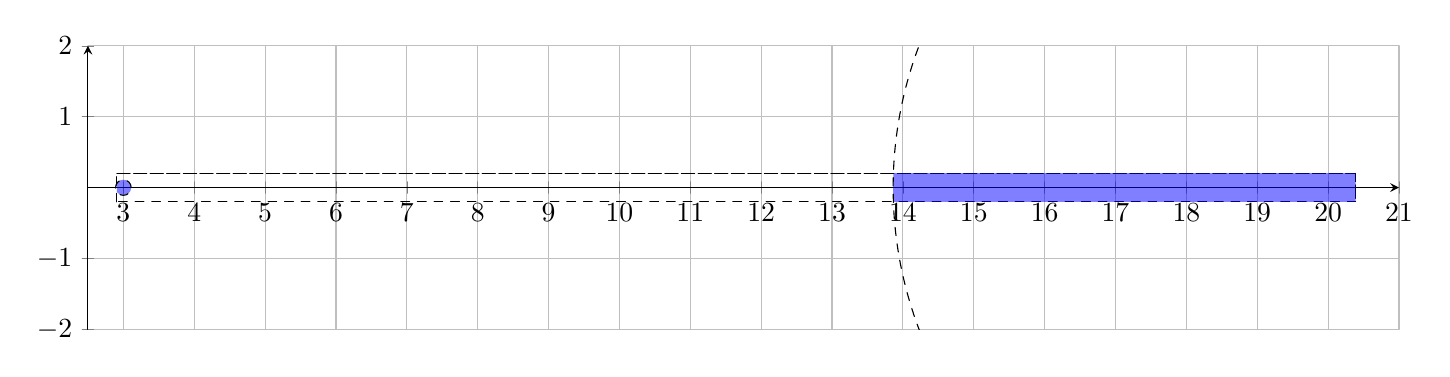
\begin{tikzpicture}[line cap=round,line join=round,>=triangle 45,x=0.9cm,y=0.9cm]
    \begin{axis}[
    x=0.9cm,y=0.9cm,
    axis lines=middle,
    ymajorgrids=true,
    xmajorgrids=true,
    xmin=2.5,
    xmax=21.0,
    ymin=-2.0,
    ymax=2.0,
    xtick={3.0,4.0,...,21.0},
    ytick={-2.0,-1.0,...,2.0},]
        \clip(2.5,-2.) rectangle (21.,2.);
        \draw[dashed] (2.909090909090909,-0.2) -- (2.909090909090909,0.2) -- (20.38888888888889,0.2) -- (20.38888888888889,-0.2) -- cycle;
        \draw[dashed] (2.909090909090909,-0.2)-- (2.909090909090909,0.2);
        \draw[dashed] (2.909090909090909,0.2)-- (20.38888888888889,0.2);
        \draw[dashed] (20.38888888888889,0.2)-- (20.38888888888889,-0.2);
        \draw[dashed] (20.38888888888889,-0.2)-- (2.909090909090909,-0.2);
        \begin{scope}
            \clip (2.909090909090909,-0.2) rectangle (20.38888888888889, 0.2); 
            \fill[blue, fill opacity=0.5]  (3.,0.) circle (0.09910020355833914cm);
            \fill[blue, fill opacity=0.5]  (19.5,0.) circle (5.073897468290155cm);
        \end{scope}
        \draw[dashed]  (3.,0.) circle (0.09910020355833914cm);
        \draw[dashed]  (19.5,0.) circle (5.073897468290155cm);
    \end{axis}
\end{tikzpicture}
    }
\end{figure}
\vfill
Hello?

\end{document}